\documentclass[a4paper,10pt]{report}
\usepackage[utf8]{inputenc}

\usepackage{tikz}
\usetikzlibrary{arrows}

\usepackage{graphicx}

% Syntax trees
\usepackage{tikz-qtree}

% Subfigures
\usepackage{subfigure}

\usepackage{color}

% Chinese
\usepackage{CJKutf8}

% Title Page
\title{Stanford University - CS224N - Natural Language Processing}
\author{Vassilis Moustakas}


\begin{document}
\maketitle

%\begin{abstract}
%\end{abstract}

\chapter*{Introduction}

\section*{Natural Language Processing and Understanding}
Natural language understanding is as old as people thinking about computers or robots and using natural language to communicate with the machine.

Computer scientists and programmers always wanted to deal with perfectly defined, unambigous constructs which is not the case for natural language. The dominant reaction of the computing industry was to avoid the problem by just saying that natural language emph{is not the right thing for machines} and deal with just machine understandable information in the form of XML, UI components, Semantic Web e.t.c. (invest on human cleverness over machine cleverness)

Goals of the field of NLP: Computers would be a lot more useful if they could understand natural language since a lot of information posessed by human beings is in that unstructured form  (i.e., e-mail, libraries, speech e.t.c.). Works out the hard problems to make computers to be able to understand, process and produce human languages (even learn them).

Natural language is the most primitive UI

Dave Bowman: Open the pod bay doors, HAL.
HAL: I'm sorry Dave. I'm afraid I can't do that.
(c.f. also false Maria in Metropolis - 1926)

Far reaching:
\begin{itemize}
 \item True text understanding and interpretation
 \item Real time participation in spoken dialogs
 \item High quality machine translation
\end{itemize}

Down to earth :
\begin{itemize}
 \item Finding the price of products on the Web
 \item Context sensitive spelling correction
 \item Analysing readin level or authorship statistically
 \item Sentiment detection about product or stocks
 \item Extracting names, facts or relations from documents
\end{itemize}

NLP tries to identify (at least some of) the hidden structure and meaning of language, not just string processing like simple keyword matching in search engines or conversion of a sound stream to a string of words in speech recognition systems.

\section*{History of NLP}
In the \emph{1950s} and withing the Cold War context, huge amount of funding was directed towards early NLP research, particularly \emph{Machine Translation (MT)}, starting with the \emph{Georgetown experiment}. The success of the experiment let, then, researchers assert that Machine Translation will be a solved problem within the next three to five years. They were proven false. At the time, there was neither the technology nor the science available for things to go far. Machines used back then were less powerful than contemporary pocket calculators and there was little understanding of how human languages really work (syntax, semantics, pragmatics e.t.c). Most of the models of language that were built during the 30's, 40's and early 50's were actually modeling language as finite state machines which was later proven completely inadequate for the complexity of human languages\footnote{The development of the Chomsky-Schützenberger hierarchy proved that the complexity of the structure of human languages was clearly beyond that of context-free languages.}. As a result, systems built during the \emph{1960s} mostly did some kind of direct word-for-word replacement. Ten years after the Georgetown experiment, the famous \emph{1966} report by the Automatic Language Processing Advisory Committee (ALPAC) evaluated the progress in computational linguistics as unsatisfactory and deemed the Machine Translation problem as intractable and not worthy of serious scientific investigation which eventually caused the U.S. Government to reduce its funding dramatically. The conclusion was that research should be focusing on understanding language instead. The years \emph{1966-1975} are considered the Machine Translation winter, during which no real steps where made to advance the field. Then, there has started to be a resurgence in parts of the world that needed translation more like Europe and Japan (domain specific rule-based systems) during the period of \emph{1975-1985} which then led to a gradual resurgence in the US as well (\emph{1985-1995}). But, generaly, by the late \emph{1990s} no one was really doing any interesting research on Machine Translation but rather on other areas of Natural Language Processing like \emph{parsing}, \emph{information extraction} etc. What really turned the world around was when IBM machine translation models
that were produced and \emph{Statistical Machine Translation (SMT)} started to be hotly pursued.

What have happened between the ALPEC report, when MT was deemed impossible and now? A lot of things:
\begin{itemize}
 \item The \textbf{need} for machine translation not only did not go away but increased due to various economic and political reasons. For example, internationalization of trade and multinational companies or the greater unification of countries like the European Union or Hong Kong becoming part of China.
 \item The \textbf{expectations} changed. In the past, the target group for MT was mainly document producers that required a perfect translation output (i.e., a product's user manual). Recently new oportunities emerged where a \emph{rough translation} can still enable billions of users browse the Web-sites, play the games or do on-line chat in languages other than hers. This model of MT is often refered to as \emph{Computer-Aided Human Translation (CAHT or CAT)}.
  \item The \textbf{technology} has become significantly better.
 \item The abundance of \textbf{data} available (WWW or any other data in digital form) nowadays, often refered to as \emph{Big Data}, made things a lot more possible.
\end{itemize}

\section*{Inverse problems and Natural Language Undersanding}

Natural language understanding fall below the kind of problems that people often call inverse problems. An \emph{inverse problem} is a general framework that is used to convert observed measurements into information about a physical object or system. The complementary problem is called \emph{direct problem}. To better understand the notions, let's consider a movie analogy. Generating realistic graphics of a movie scene is the direct problem. You have a model of the objects you want to appear in it and you genearate the graphics. On the other hand, using computer vision to ``see'' a surface frame picture and try to ``understand'' and reconstruct the objects that appear in the scene is a facet of the inverse problem. Direct problems are often the easy problems whereas the inverse are the difficult ones.

\subsection*{Ambiguity}
Natural language understanding difficulty as an inverse problem stems from the fact that the hidden structure of a human language is hugely ambiguous. Take for example the following sentence:
\begin{quote}
 \textit{Fed raises interest rates 0.5\% in effort to control inflation (NYT headline 17 May 2000).}
\end{quote}
The meaning of the sentence sounds pretty obvious if you read it casually from the economic section of the newspaper. Doesn't look like there is ambiguity at all. Unfortunately, if you look closely, you will find out this is not actually the case.

Take, for example, the syntactic tree shown in Figure~\ref{ambiguity:0} which is what the casual reader will construct in her head while reading the previous example sentence.

\begin{figure}[ht]
\centering
\resizebox{\textwidth}{!}{%
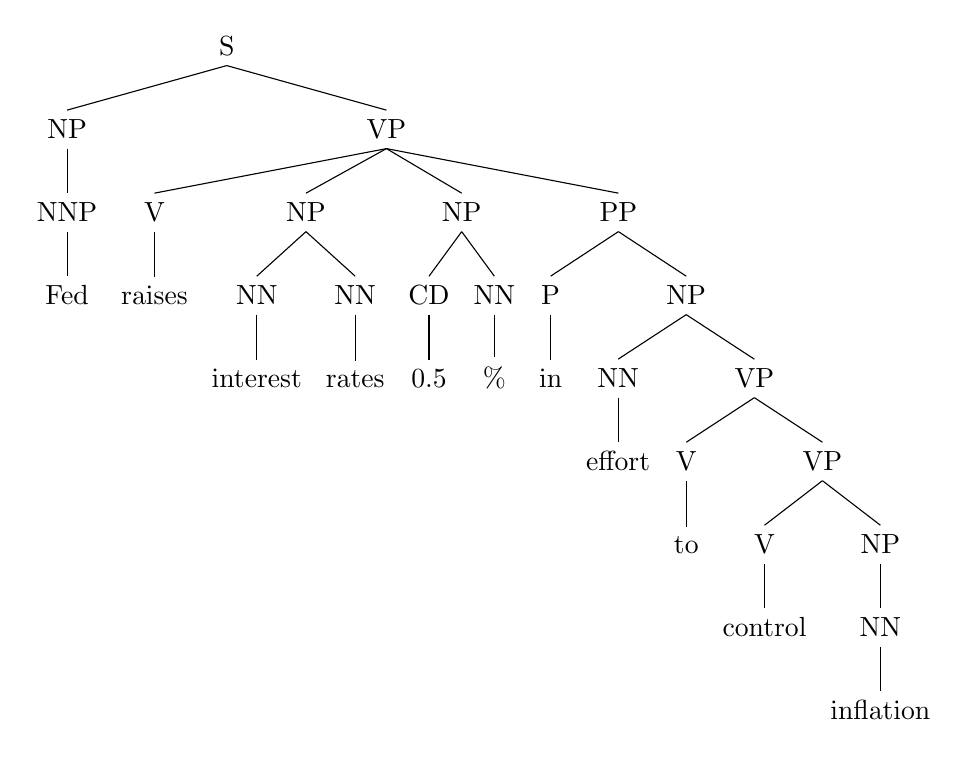
\begin{tikzpicture}
\Tree [.S
  [.NP
    [.NNP Fed ]
  ]
  [.VP
    [.V raises ]
    [.NP
      [.NN interest ]
      [.NN rates ]
    ]
    [.NP
      [.CD 0.5 ]
      [.NN \% ]
    ]
    [.PP
      [.P in ]
      [.NP
        [.NN effort ]
        [.VP
          [.V to ]
          [.VP
            [.V control ]
            [.NP
              [.NN inflation ]
            ]
          ]
        ]
      ]
    ]
  ]
]
\end{tikzpicture}
}
\caption{Casual reader syntactic tree construct.}
\label{ambiguity:0}
\end{figure}

In English there is a fundamental fact that there are tons of words that can act both as verbs and nouns. This means that the above syntactic structure, though obvious it is not the only one possible. This introduces a ton of \emph{syntactic ambiguity} that makes understanding of the sentece very difficult for a machine. Checkout the different possible syntactic trees shown in Figure~\ref{ambiguity:123}.

\begin{center}
\begin{table}
\begin{tabular}{ c c c c c c c }
  \multicolumn{6}{c}{Part of speech} & Syntactic attachment\\
  & & \textbf{VB} & & & & \\
  & \textbf{VBZ} & \textbf{VBP} & \textbf{VBZ} & & & \\
  \textbf{NNP} & \textbf{NNS} & \textbf{NN} & \textbf{NNS} & \textbf{CD} & \textbf{NN} & \\
  Fed & raises & interest & rates & 0.5 & \% & in effort to control inflation \\
\end{tabular}
\caption{Part of speech and syntactic attachement ambiguities}
\end{table}
\end{center}

\begin{figure}[ht]
\centering
\subfigure[] {
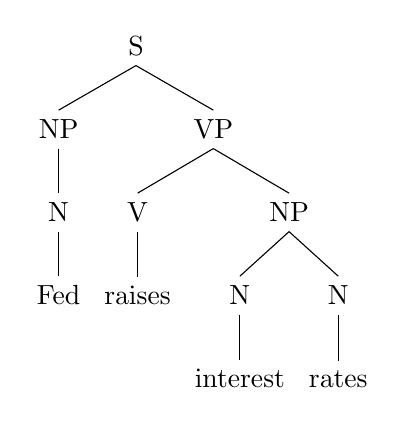
\begin{tikzpicture}
\Tree [.S
  [.NP
    [.N Fed ]
  ]
  [.VP
    [.V raises ]
    [.NP
      [.N interest ]
      [.N rates ]
    ]
  ]
]
\end{tikzpicture}
\label{ambiguity:1}
}\qquad\qquad
\subfigure[] {
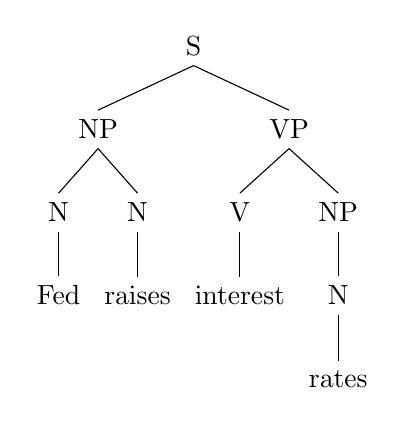
\begin{tikzpicture}
\Tree [.S
  [.NP
    [.N Fed ]
    [.N raises ]
  ]
  [.VP
    [.V interest ]
    [.NP
      [.N rates ]
    ]
  ]
]
\end{tikzpicture}
\label{ambiguity:2}
}\qquad\qquad
\subfigure[] {
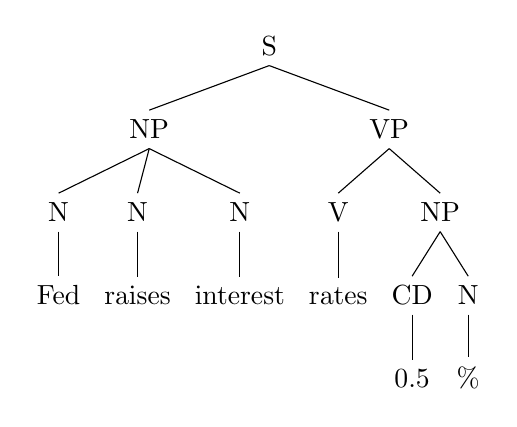
\begin{tikzpicture}
\Tree [.S
  [.NP
    [.N Fed ]
    [.N raises ]
    [.N interest ]
  ]
  [.VP
    [.V rates ]
    [.NP
      [.CD 0.5 ]
      [.N \% ]
    ]
  ]
]
\end{tikzpicture}
\label{ambiguity:3}
}
\caption{The bad effects of V/N ambiguity.}
\label{ambiguity:123}
\end{figure}

Apart from syntactic there can also be interpretation ambiguities above word level, called \emph{semantic ambiguity}. For example, \emph{word sense ambiguity} of the word ``Fed'' that in this case means ``Federal Reserve Board'' but in others could refer to an ``FBI agent'' or to the past tense of the verb ``to feed''. Also ``interest'' might have different meanings from ``something that you like'' to ``having a stake at a company'' or ``a rate that you pay''. Moreover, towards the end of the example sentence, there are the prepositional phrase ``in effort'' and the infinitive phrase ``to control inflation''. Whenever you have those kind of phrases you have ambiguity as to what they modify. For example, does ``in effort'' modify the noun phrase ``0.5\%'' or the verb ``raises''? This is what linguists call \emph{syntactic attachement ambiguity}.

In newspaper headlines a lot of functional words are omited which result more often in ambiguity. Following are some more funny examples:
\begin{quote}
 \textit{Ban on Nude Dancing on Governor's Desk. (prepositional phrase attach - syntactic attachement ambiguity)} \\
 \textit{Iraqi Head Seeks Arms. (sense extension - word sense ambiguity)} \\
 \textit{Juvenile Court to Try Shooting Defendant. (syntactic attachement ambiguity)} \\
 \textit{Teacher Strikes Idle Kids.} \\
 \textit{Stolen Painitng Found by Tree. (semantic interpretation ambiguity of ``by Tree'')} \\
 \textit{Local Hish School Dropouts Cut in Half.} \\
 \textit{Red Tape Holds Up New Bridges.} \\
 \textit{Clinton Wins on Budget but More Lies Ahead.} \\
 \textit{Hospitals Are Sued by 7 Foot Doctors.} \\
 \textit{Kids Make Nutritious Snacks.} \\
 \textit{Minister Accused Of Having 8 Wives In Jail.} \\
\end{quote}

\subsubsection*{Reference Resolution}

Where is {\color{red}A Bug’s Life} playing in {\color{red}Mountain View} ?

A Bug’s Life is playing at the Century 16 Theater.

When is {\color{green}it} playing {\color{green}there} ?

It’s playing at 2pm, 5pm, and 8pm.

OK. I’d like 1 {\color{blue}adult} and 2 {\color{blue}children} for {\color{blue}the first show}. How much would {\color{green}that} cost?

But we need {\color{red}domain knowledge}, {\color{green}discourse knowledge}, {\color{blue}world knowledge}, linguistic knowledge.

Natural language understanding is extremely difficult, sometimes being considered as one of the AI-complete problems. The reason is that natural language is highly ambiguous at all levels. It depends on making complex and subtle use of context, both context of the rest of the sentence, prior discourse or even reasoning about the World.

On the other hand, has been proven that we can do a surprisingly good job for a lot of tasks only through simple approximations of knowledge about language and context and the World. For example, in context-sensitive spelling correction, we can simply look through large amounts of text and count how often diffent spellings appear in different contexts and use that info to infer the way something should be spelled when a gap appears in a similar context.

Thus, the answer to Natural Language Processing has recently been the use of probabilistic models. The idea behind it is that even though we may have uncertain knowledge about the language, context and the World, we can still combine all the evidence that we know and combine it together to give the best prediction or understanding or interpretation of what was said. This is what Probablity Theory in general is all about and it works rather nicely for a lot of natural language problems. Interestingly enough, probabilistic methods have been used, since a lot time, by electrical engineers in signal processing for another field of natuaral language, that of speech recognition, which is essentialy the way to reconstruct words from an uncertain audio signal.

\chapter*{Machine Translation}

\section*{Approaches to Machine Translation}
There are different approaches to Machine Translation based on how deep you are going in attempting to translate as shown by the \emph{Vauquois Triangle} of Figure~\ref{mt:vauquois}. The general idea is that we do some processing of the source text and at some point we convert across to the other language to get the target text. The possibilities are:
\begin{itemize}
 \item \emph{Direct}: Extremely minimal processing such as tokenizaton and/or normalization and then go straight at the word level to the target language. That is what was done in the 1950s but still this is what it is also what is done with Statistical Machine Translation. In the latter case, statistics help to do that a lot better.
 \item \emph{Transfer}: Atempt to understand more about the source text. For example do, syntactic analysis to produce the syntactic structure of the source text and then do \emph{syntactic transfer} attempt to produce the syntactic tree for the target language and ultimately generate the target text. That is a contemporary area of research called \emph{syntax-based Statistical Machine Translation}. During the 1980s there was an attempt to go even deeper by trying to understand the language in a semantic level and generate the target text through \emph{semantic transfer}.
 \item \emph{Interlingual}: Also during the 1980s, huge effort was made to define a universal semantic structure, common for all languages, usually reffered to as the \emph{interlingua}. The idea is to translate from the source language to interlingua and then from interlingua to the target language. This approach is appealing because with the direct or transfer approaches you need to build order $n^2$ translation systems. For example, having one system that does English to German and one that does German to Greek doesn't mean you can do English to Greek; we need to build a dedicated translator. With interlingua you need to build order $n$ systems to translate between every language pair. This did not go far though. Perhaps it was a false idea from the start since the problem is that different languages have all kinds of distinctions, and ways of looking at the World that are of their own and aren’t reproduced in other languages. This means that trying to design an interlingua that works for every language, that means you have to put into the interlingua the complexities of every individual language, and that makes it a very hard goal to get to. 
\end{itemize}


\begin{figure}[ht]
\centering
\resizebox{\textwidth}{!}{%
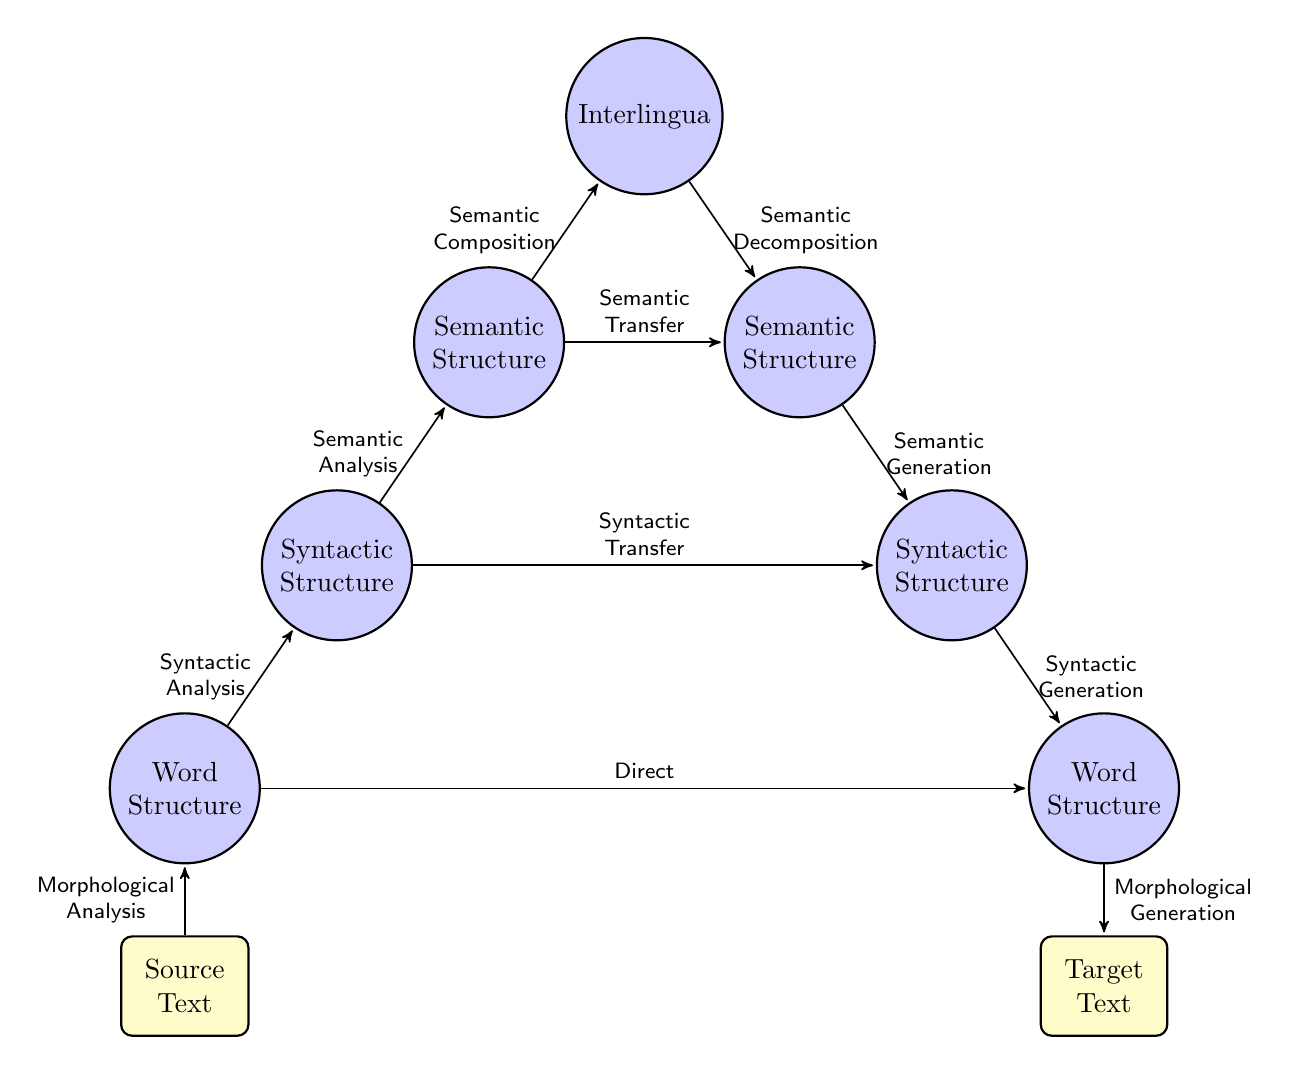
\begin{tikzpicture}[
%  font=\sffamily,
  every matrix/.style={ampersand replacement=\&,column sep=0cm,row sep=0.9cm},
  source/.style={draw,thick,rounded corners,fill=yellow!20,inner sep=.3cm},
  target/.style={draw,thick,rounded corners,fill=yellow!20,inner sep=.3cm},
  process/.style={draw,thick,circle,fill=blue!20},
  to/.style={->,>=stealth',shorten >=1pt,semithick,font=\sffamily\footnotesize},
  every node/.style={align=center}]

  % Position the nodes using a matrix layout
  \matrix{
    \& \& \& \node[process] (interlingua) {Interlingua}; \\
  
    \& \& \node[process] (semanticsource) {Semantic\\Structure};
    \& \& \node[process] (semantictarget) {Semantic\\Structure}; \\
  
    \& \node[process] (syntacticsource) {Syntactic\\Structure};
    \& \& \& \& \node[process] (syntactictarget) {Syntactic\\Structure}; \\
  
    \node[process] (wordsource) {Word\\Structure};
    \& \& \& \& \& \& \node[process] (wordtarget) {Word\\Structure}; \\
  
    \node[source] (sourcetext) {Source\\Text};
    \& \& \& \& \& \& \node[target] (targettext) {Target\\Text}; \\
  };

  % Draw the arrows between the nodes and label them.
   \draw[to] (semanticsource) -- node[midway,left] {Semantic\\Composition} (interlingua);
   \draw[to] (interlingua) -- node[midway,right] {Semantic\\Decomposition} (semantictarget);
   \draw[to] (semanticsource) -- node[midway,above] {Semantic\\Transfer} (semantictarget);
   \draw[to] (syntacticsource) -- node[midway,left] {Semantic\\Analysis} (semanticsource);
   \draw[to] (semantictarget) -- node[midway,right] {Semantic\\Generation} (syntactictarget);
   \draw[to] (syntacticsource) -- node[midway,above] {Syntactic\\Transfer} (syntactictarget);
   \draw[to] (wordsource) -- node[midway,left] {Syntactic\\Analysis} (syntacticsource);
   \draw[to] (syntactictarget) -- node[midway,right] {Syntactic\\Generation} (wordtarget);
   \draw[to] (wordsource) -- node[midway,above] {Direct} (wordtarget);
   \draw[to] (sourcetext) -- node[midway,left] {Morphological\\Analysis} (wordsource);
   \draw[to] (wordtarget) -- node[midway,right] {Morphological\\Generation} (targettext);
\end{tikzpicture}
}
\caption{The Vauquois Triangle.}
\label{mt:vauquois}
\end{figure}

\subsection*{Statistical Machine Translation}

\begin{quotation}
 \textit{Statistical machine translation (SMT) is a machine translation paradigm where translations are generated on the basis of statistical models whose parameters are derived from the analysis of bilingual text corpora.}
\end{quotation}

The essential answer to how to do MT by statistical methods is shown in Figure~\ref{mt:rosetta}. The \emph{Rosseta Stone} is the reason decoding of Hieroglyphics happened. The (correct) assumption was that the stone had the same text carved on it in three different languages, namely Hieroglyphics at the upper section, Demotic Coptic at the center and Greek at the lower section. This is called \emph{parallel text} and can help induce statistical models of Machine Translation. For a Spanish to English translation context we can come up with rules like: \textit{every time one sees ``banco'', translation is ``bank'' or ``bench'' ... If it’s ``banco de...'', it always becomes ``bank'', never ``bench''}.

There are a lot of sources for \emph{parallel text} around us like instruction manuals, Hong Kong legislation, Macao legislation, Canadian parliament hansards, United Nations reports, official journal of the European Communities etc.

\begin{figure}[ht!]
\centering
\resizebox{\textwidth}{!}{%
\includegraphics[]{img/rosetta.jpg}
}
\caption{The Rosetta Stone \label{overflow}}
\label{mt:rosetta}
\end{figure}


 containing  A simple caption

\begin{CJK*}{UTF8}{gbsn}
美国关岛国际机场及其办公室均接获一名自称沙地阿拉伯富商拉登等发出的电子邮件,威胁将会向机场等公众地方发动生化袭击後,关岛经保持高度戒备。
\end{CJK*}

The U.S. island of Guam is maintaining a high state of alert after the Guam airport and its offices both received an e-mail from someone calling himself the Saudi Arabian Osama bin Laden and threatening a biological/chemical attack against public places such as the airport. 

\end{document}          
